\documentclass{scrartcl}
\usepackage{amsmath}
\usepackage{amssymb}
\usepackage{unicode-math}
\setmathfont{XITS Math}
\usepackage{tikz}
\usetikzlibrary{positioning}

\newcommand{\selection}{\sigma}
\newcommand{\projection}{\pi}
\newcommand{\rename}{\rho}
\newcommand{\join}{\Join}
% \fullouterjoin defined by unicode-math
\newcommand{\semijoin}{\ltimes}
\newcommand{\groupby}{\Gamma}

\newcommand{\mtt}[1]{\text{\texttt{#1}}}

\setlength{\parindent}{0pt}

\begin{document}

\section*{Exercise 1}

\subsection*{1.}

Consider the following join graph:

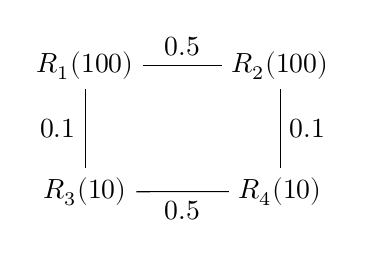
\begin{tikzpicture}
    \node (R1) {$R_1 (100)$};
    \node (R2) [right=of R1] {$R_2 (100)$};
    \node (R3) [below=of R1] {$R_3 (10)$};
    \node (R4) [below=of R2] {$R_4 (10)$};
    \draw (R1) to node [above] {$0.5$} (R2);
    \draw (R1) to node [left] {$0.1$} (R3);
    \draw (R2) to node [right] {$0.1$} (R4);
    \draw (R3) to node [below] {$0.5$} (R4);
\end{tikzpicture}

Here GOO would result in the query $((R_3 \join R_4) \join R_2) \join R_1$. Its
cost is:
\begin{align*}
&\phantom{{}={}} C_{out}((R_3 \join R_4) \join R_2) \join R_1) \\
&= |(R_3 \join R_4) \join R_2) \join R_1| + C_{out}((R_3 \join R_4) \join R_2) +
C_{out}(R_1) \\
&= 2500 + |(R_3 \join R_4) \join R_1| + C_{out}(R_3 \join R_4) + C_{out}(R_2) \\
&= 2500 + 500 + |R_3 \join R_4| + C_{out}(R_3) + C_{out}(R_4) \\
&= 2500 + 500 + 50 \\
&= 3050
\end{align*}
But the optimal tree is $(R_1 \join R_3) \join (R_2 \join R_4)$. Its cost is:
\begin{align*}
&\phantom{{}={}} C_{out}((R_1 \join R_3) \join (R_2 \join R_4)) \\
&= |(R_1 \join R_3) \join (R_2 \join R_4)| + C_{out}(R_1 \join R_3) +
C_{out}(R_2 \join R_4) \\
&= 2500 + |R_1 \join R_3| + |R_2 \join R_4| \\
&= 2500 + 100 + 100 \\
&= 2700
\end{align*}

\subsection*{2.}

We have to pick every node as root node and build the minimum spanning tree.

\subsubsection*{Root $R_1$}

\begin{minipage}{0.8\textwidth}
\begin{minipage}[c]{0.5\textwidth}
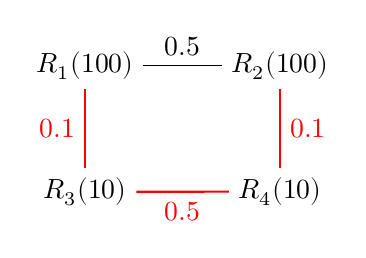
\begin{tikzpicture}
    \node (R1) {$R_1 (100)$};
    \node (R2) [right=of R1] {$R_2 (100)$};
    \node (R3) [below=of R1] {$R_3 (10)$};
    \node (R4) [below=of R2] {$R_4 (10)$};
    \draw (R1) to node [above] {$0.5$} (R2);
    \draw [red,thick] (R1) to node [left] {$0.1$} (R3);
    \draw [red,thick] (R2) to node [right] {$0.1$} (R4);
    \draw [red,thick] (R3) to node [below] {$0.5$} (R4);
\end{tikzpicture}
\end{minipage}
\begin{minipage}[c]{0.5\textwidth}
\begin{tabular}{llllll}
R & n & s & C & T & rank \\ \hline
3 & 10 & 0.1 & 1 & 1 & 0 \\
4 & 10 & 0.5 & 5 & 5 & 0.8 \\
2 & 100 & 0.1 & 10 & 10 & 0.9
\end{tabular}
\end{minipage}
\end{minipage}

This results in the following query: $((R_1 \join R_3) \join R_4) \join R_2$.
Its $C_{out}$ cost is 3100.


\subsubsection*{Root $R_2$}

\begin{minipage}{0.8\textwidth}
\begin{minipage}[c]{0.5\textwidth}
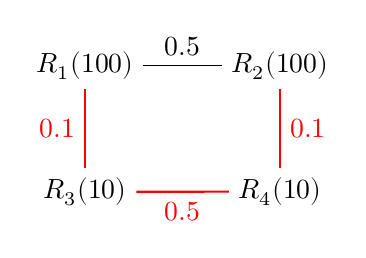
\begin{tikzpicture}
    \node (R1) {$R_1 (100)$};
    \node (R2) [right=of R1] {$R_2 (100)$};
    \node (R3) [below=of R1] {$R_3 (10)$};
    \node (R4) [below=of R2] {$R_4 (10)$};
    \draw (R1) to node [above] {$0.5$} (R2);
    \draw [red,thick] (R1) to node [left] {$0.1$} (R3);
    \draw [red,thick] (R2) to node [right] {$0.1$} (R4);
    \draw [red,thick] (R3) to node [below] {$0.5$} (R4);
\end{tikzpicture}
\end{minipage}
\begin{minipage}[c]{0.5\textwidth}
\begin{tabular}{llllll}
R & n & s & C & T & rank \\ \hline
4 & 10 & 0.1 & 1 & 1 & 0 \\
3 & 10 & 0.5 & 5 & 5 & 0.8 \\
1 & 100 & 0.1 & 10 & 10 & 0.9 \\
\end{tabular}
\end{minipage}
\end{minipage}

This results in the following query: $((R_2 \join R_4) \join R_3) \join R_1$.
Its $C_{out}$ cost is 3100.


\subsubsection*{Root $R_3$}

\begin{minipage}{0.8\textwidth}
\begin{minipage}[c]{0.5\textwidth}
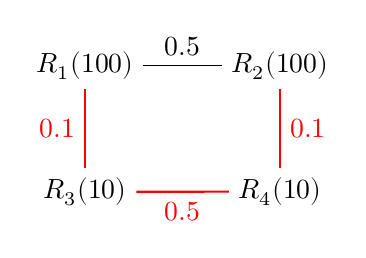
\begin{tikzpicture}
    \node (R1) {$R_1 (100)$};
    \node (R2) [right=of R1] {$R_2 (100)$};
    \node (R3) [below=of R1] {$R_3 (10)$};
    \node (R4) [below=of R2] {$R_4 (10)$};
    \draw (R1) to node [above] {$0.5$} (R2);
    \draw [red,thick] (R1) to node [left] {$0.1$} (R3);
    \draw [red,thick] (R2) to node [right] {$0.1$} (R4);
    \draw [red,thick] (R3) to node [below] {$0.5$} (R4);
\end{tikzpicture}
\end{minipage}
\begin{minipage}[c]{0.5\textwidth}
\begin{tabular}{llllll}
R & n & s & C & T & rank \\ \hline
4 & 10 & 0.5 & 5 & 5 & 0.8 \\
1 & 100 & 0.1 & 10 & 10 & 0.9 \\
2 & 100 & 0.1 & 10 & 10 & 0.9
\end{tabular}
\end{minipage}
\end{minipage}

This results in the following query: $((R_3 \join R_4) \join R_1) \join R_2$.
Its $C_{out}$ cost is 3050.


\subsubsection*{Root $R_4$}

\begin{minipage}{0.8\textwidth}
\begin{minipage}[c]{0.5\textwidth}
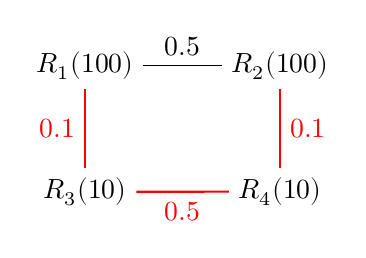
\begin{tikzpicture}
    \node (R1) {$R_1 (100)$};
    \node (R2) [right=of R1] {$R_2 (100)$};
    \node (R3) [below=of R1] {$R_3 (10)$};
    \node (R4) [below=of R2] {$R_4 (10)$};
    \draw (R1) to node [above] {$0.5$} (R2);
    \draw [red,thick] (R1) to node [left] {$0.1$} (R3);
    \draw [red,thick] (R2) to node [right] {$0.1$} (R4);
    \draw [red,thick] (R3) to node [below] {$0.5$} (R4);
\end{tikzpicture}
\end{minipage}
\begin{minipage}[c]{0.5\textwidth}
\begin{tabular}{llllll}
R & n & s & C & T & rank \\ \hline
3 & 10 & 0.5 & 5 & 5 & 0.8 \\
1 & 100 & 0.1 & 10 & 10 & 0.9 \\
2 & 100 & 0.1 & 10 & 10 & 0.9
\end{tabular}
\end{minipage}
\end{minipage}

This results in the following query: $((R_4 \join R_3) \join R_1) \join R_2$.
Its $C_{out}$ cost is 3050.

\subsubsection*{Conclusion}

The IKKBZ heuristics give us a plan with a cost of 3050 which is the same as
GOO but of course not optimal.

\end{document}
